\documentclass[conference]{IEEEtran}
\IEEEoverridecommandlockouts
\usepackage{cite}
\usepackage{amsmath,amssymb,amsfonts}
\usepackage{algorithmic}
\usepackage{graphicx}
\usepackage{textcomp}
\usepackage{xcolor}
\usepackage{multirow}
\usepackage{makecell}
\usepackage{float}
\usepackage{multicol}
\usepackage{subcaption}

\def\BibTeX{{\rm B\kern-.05em{\sc i\kern-.025em b}\kern-.08em
    T\kern-.1667em\lower.7ex\hbox{E}\kern-.125emX}}

\begin{document}

\title{Blood cells image segmentation and counting using deep transfer learning }

\author{
\IEEEauthorblockN{1\textsuperscript{st} Gharbi Aghiles $^1$}
\and
\IEEEauthorblockN{2\textsuperscript{nd} Neggazi Mohamed Lamine $^1$}
\and
\IEEEauthorblockN{3\textsuperscript{rd} Touazi Faycal $^1$}
\and
\IEEEauthorblockN{4\textsuperscript{th} Gaceb Djamel $^1$}\and
\IEEEauthorblockN{5\textsuperscript{th} Yagoubi Mohamed Riad $^1$\\
\textit{ $^1$ University M’hamed Bougara, Independence Avenue, 35000, 
Boumerdes, Algeria\\
\{a.gharbi, a.neggazi, f.touazi, d.gaceb, md.yagoubi\}@univ-boumerdes.dz}}}
\maketitle
\vspace*{-0.8cm}
\begin{abstract}

In this paper, we present a two-step automatic blood cell counting approach for accurately and efficiently determining the complete blood count (CBC). The approach involves using two convolutional neural networks (CNNs) for the segmentation of red blood cells, white blood cells, and platelets, and then applying three different algorithms (Watershed, Connected Component Labeling, and Circle Hough Transform) to count the cells present in the masks produced by the CNNs. We also introduce a loss function for the Circle Hough Transform algorithm to further improve its accuracy. Our approach shows good results compared to other methods in the literature and has the potential to significantly reduce the time and effort required for manual blood cell counting.
\end{abstract}

\begin{IEEEkeywords}
Blood cell segmentation, Blood cell counting, U-net, SegNet, deep learning 
\end{IEEEkeywords}

\section{Introduction}
The complete blood count (CBC) is a routine medical test that provides important information about the cells present in the blood, including red blood cells, white blood cells, and platelets. Accurate and reliable CBC results are essential for the diagnosis and treatment of a wide range of medical conditions, including infections, anemias, and cancers.

Traditionally, CBCs have been performed manually by trained laboratory personnel using microscopes and specialized equipment. However, this method is time-consuming and requires a high level of concentration and skill. There is also a lack of standardization among different laboratories, which can lead to inconsistent results.

To address these limitations, various automated blood cell counting systems have been developed in recent years \cite{asgari2021deep}. These systems often use machine learning algorithms and image analysis techniques to accurately and efficiently determine the CBC.

In this paper, we present a two-step automatic blood cell counting approach as follow:
\begin{itemize}
    \item \textbf{The segmentation:} where we need to segment the image and remove the noise to get a clear mask on which we are going to perform the counting. In this phase we are comparing between two convolutional neural networks U-Net and SegNet.
    \item \textbf{The counting:} in which we will take the output mask (and edge-mask for red blood cells) from the first phase and apply counting algorithms on it. We used 3 algorithms to count the cells: Watershed, Connected Component Labeling, Circle Hough transform.\\
\end{itemize}

The organization of this paper is as follows: Related work describes the research in the area of blood cells segmentation and counting, Data Description describes the dataset used in the proposed approach, Methodology describes the proposed approach. Finally, the last section describes the results of the proposed approach, 

\section{Related Work}

Bhavnani et al. \cite{bhavnani2016segmentation} have developed a method for segmenting and counting red blood cells (RBC), White blood cells (WBC) and platelets which is also called complete blood count (CBC), by using Otsu’s threshold and morphological operations as a segmentation method, and for counting they are performing a comparison between two methods: the watershed algorithm and Circular Hough Transform.

Guiliang, FENG et al.\cite{guiliang2016microscopic} have a developed an algorithm that segments and counts cell images based on image definition, a Discrete Cosine Transform (DCT) is applied, which was proposed by N. Ahmed and Rao in 1974 \cite{ahmed1974discrete}. Instead of the traditional watershed approach, the DCT method showed better results in comparison. However, there is a drawback to this approach, because this algorithm depends on image definition it relies on well focused images, consequently, when the images are out of focus the segmentation and counting is not reliable. But despite that drawback, it achieved a relatively high accuracy of over 90\% which is better that the watershed method.

In a study by K. Sudha and P. Geetha \cite{SUDHA2020639}, a two-stage framework was developed to segment leukocytes (a type of white blood cell) using an edge strength-based Grabcut method in the first stage and to count the cells using the gradient circular hough transform (GCHT) method in the second stage. The ALL-IDB \cite{labati2011all} and Cellavision \cite{Zheng2018} datasets were used in the experimental phase.

Carlos X. Hern{\'{a}}ndez et al. \cite{DBLP:journals/corr/abs-1802-10548} have used a convolutional neural network (CNN) using a feature pyramid network (FPN) combined with a VGG style neural network for segmenting and counting of cells in a given microscopy image.

Tran, Thanh and Minh et al. \cite{tran2019blood} have developed a method for segmenting and counting RBC and WBCs by using the SegNet model initialized with weights from a pre-trained VGG-16 model, for the counting they first apply Distance transform with 4 different distance metrics, then they apply binary dilation. Finally, the connected component labeling algorithm was applied to count the number of separated cells in the images mask. 

Yan Kong et al. \cite{Kong:20} created a two-stage framework that utilizes parallel modified U-Nets and a seed guided water-mesh algorithm for automatic segmentation and counting of yeast cells. This framework is utilized to assess the living conditions and survival of yeast cells in experimental settings.

Shahzad et al.  \cite{shahzad2020robust} proposed a custom convolutional encoder-decoder model that incorporates VGG-16 for feature extraction to perform semantic segmentation of cells on whole slides. This approach aims to address the issue of whole-slide cell segmentation. 

Overton, Toyah and Tucker, Allan \cite{10.1007/978-3-030-44584-3_31} have developed a method which segments and counts IDP (Internally Displaced people) and erythrocytes (red blood cells) using DO-U-Net (Dual Output U-Net) which outputs a segmentation mask and an edge mask then they subtract them to get rid of the overlapping and the touching problem.

Li, Dongming et al. \cite{li2021robust} have developed a method for segmenting blood cells by combining neural ordinary differential equations (NODEs) with U-Net networks to improve the accuracy of image segmentation.

Table \ref{resultComparingTable} outlines the main results of theses works:
% \usepackage{multirow}


\begin{table*}[h]
\centering
\resizebox{\linewidth}{!}{
\begin{tabular}{|c|c|c|c|c|c|c|c|} 
\hline
\multirow{2}{*}{\textbf{References }}                                                                        & \multicolumn{2}{c|}{\textbf{RBC }}        & \multicolumn{2}{c|}{\textbf{WBC}}                 & \multicolumn{2}{c|}{\textbf{Platelets}}  & \textbf{Dataset}   \\ 
\cline{2-7}  & \textbf{Segmentation} & \textbf{Counting} & \textbf{Segmentation} & \textbf{Counting}         & \textbf{Segmentation} & \textbf{Counting} & \\ 
\hline
%\begin{tabular}[c]{@{}c@{}}\textbf{Guiliang, FENG}\\\textbf{et al. (2016)}\end{tabular}                      & \multicolumn{6}{c|}{90\%}&N/A                                                                                                                  \\ 
\hline
\begin{tabular}[c]{@{}c@{}}\textbf{Bhavnani}\\\textbf{et al. (2016)}\end{tabular}                            & \multicolumn{4}{c|}{\begin{tabular}[c]{@{}c@{}}CHT- 92.67\%\\Watershed- 91.07\%\end{tabular}} & \multicolumn{2}{c|}{N/A}         &ALL-IDB1          \\ 
\hline
\begin{tabular}[c]{@{}c@{}}\textbf{Carlos}\\\textbf{et al. (2018)}\end{tabular}                              & \multicolumn{6}{c|}{95\%}         &BBBC005                                                                                                         \\ 
\hline
\begin{tabular}[c]{@{}c@{}}\textbf{Tran, Thanh}\\\textbf{and}\\\textbf{Minh et al.(2019)}\end{tabular}       & 93\%                  & 93.30\%           & 93\%                  & N/A                       & \multicolumn{2}{c|}{N/A}  &ALL-IDB1                 \\ 
\hline
\begin{tabular}[c]{@{}c@{}}\textbf{K. Sudha and}\\\textbf{P. Geetha (2020)}\end{tabular}                     & \multicolumn{2}{c|}{N/A }                 & 99.32\%               & 97.3\%                    & \multicolumn{2}{c|}{N/A}     &ALL-IDB1                \\ 
\hline
\begin{tabular}[c]{@{}c@{}}\textbf{Yan Kong}\\\textbf{et al. (2020)}\end{tabular}                            & \multicolumn{6}{c|}{96\%}     & Self Annotated                                                                                                              \\ 
\hline
\begin{tabular}[c]{@{}c@{}}\textbf{Shahzad}\\\textbf{et al. (2020)}\end{tabular}                             & 97.45\%               & N/A               & 93.34\%               & N/A                       & 85.11\%               & N/A         &ALL-IDB1         \\ 
\hline
\begin{tabular}[c]{@{}c@{}}\textbf{Overton, Toyah}\\\textbf{and}\\\textbf{Tucker, Allan (2020)}\end{tabular} & 98.31\%               & \multicolumn{5}{c|}{N/A}  &ALL-IDB1                                                                                      \\ 
\hline
\begin{tabular}[c]{@{}c@{}}\textbf{Li, Dongming}\\\textbf{et al. (2021)}\end{tabular}                        & \multicolumn{2}{c|}{N/A}                  & 95.3\%                & \multicolumn{3}{c|}{N/A}  &MISP\\ 
%\hline
%\textbf{Our Method}                                                                                          & 97.1\%                & 95.36\%           & 99.76\%               & 97.94\%                   & 99.46\%               & 98.58\%            \\
\hline
\end{tabular}}
\caption{Comparative table for segmentation and counting accuracy's between studied methods\label{resultComparingTable}}

\end{table*}

\section{Methodology}
In our work, we focus more on the segmentation task because it directly affects the counting accuracy. where the accuracy of the output mask and edge plays a big role in the detection of overlapping, so our main goal is to segment the overlapped cells for example in red blood cells we added an edge mask then by combining it with the mask we remove 80\% of overlapping. after the segmentation we will apply the counting algorithms (Watershed, Circle hough transform, Connected component labeling) which needs some parameter tuning in our case we did a manual tuning. we will divide this section on two: Segmentation phase and counting phase:
\subsection{Cell semantic segmentation using deep learning}
U-Net and SegNet architectures are the most used in cell segmentation tasks \cite{asgari2021deep}
(blood cell segmentation in particular).\\
In the following sections, we will briefly analyze and compare both convolutional neural network (CNN) U-Net and SegNet models with their perspective results.
And explain all the post-processing methods we used for the counting of blood cells (red, white and platelets).

\subsubsection{\textbf{DO-U-Net}}
It is a network based on a modified U-shaped CNN architecture which gives two outputs, hence the name DO-UNet. It have been extended to work with fewer training images and to yield more precise segmentation. In our case we are using DO-UNet first proposed in \cite{10.1007/978-3-030-44584-3_31} which is a modified U-Net to produce dual outputs.
Figure \ref{fig:DO-UNET} shows the DO-U-Net architecture.

\begin{figure}[ht]
\centering
    \centerline{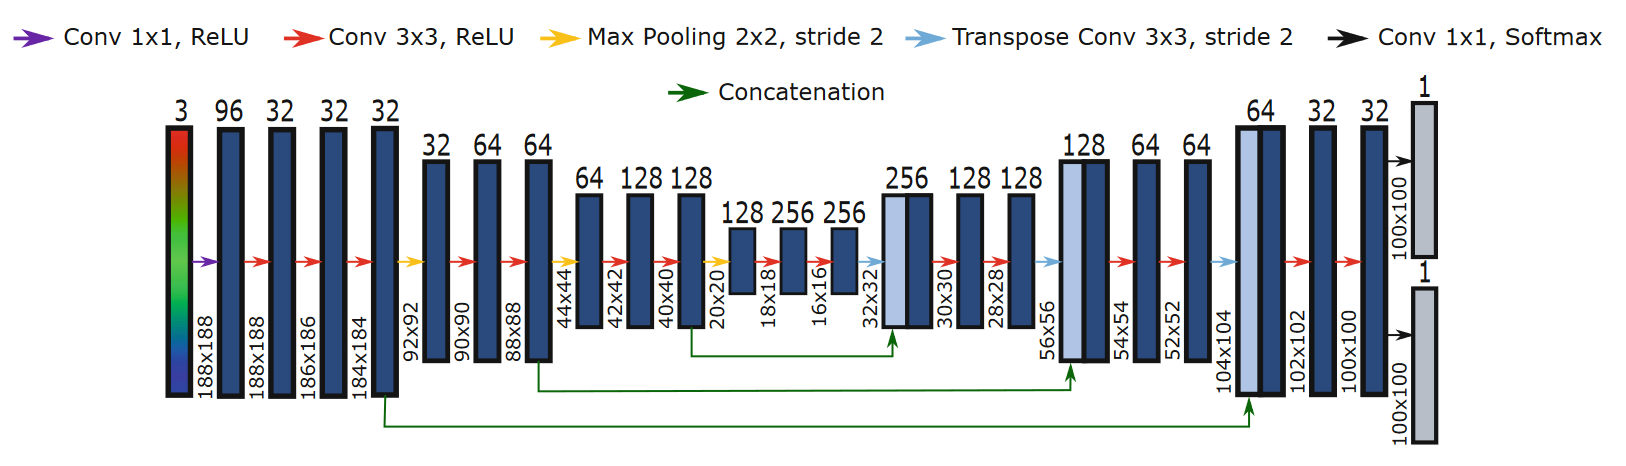
\includegraphics[width = 3.5in, height=1.6in]{../images/DO-UNET.png}}
    \caption{DO-UNet architecture}
    \label{fig:DO-UNET}
\end{figure}

\subsubsection{\textbf{SegNet}}

The SegNet neural network, first introduced in \cite{badrinarayanan2017segnet}. Is a convolutional neural network used for semantic pixel wise labeling. This problem is more commonly called semantic segmentation.

SegNet is a network with an encoder-decoder architecture. So it mainly consists of a number of convolutional layers which constitute the encoder part and second decoder part with the same principle. This network ends with a final classification layer per pixel. This architecture is illustrated in Figure \ref{segnet}.
The model we used has the 13 encoder layers obtained from the VGG16 network, and 13 decoder layers to match the same number of encoder layers. The final decoder output is fed to a multi-class soft-max classifier to produce class probabilities for each pixel independently (pixelwise) \cite{badrinarayanan2017segnet}.

\begin{figure}[ht]
\centering
  \vspace{-0.1in}
    \centerline{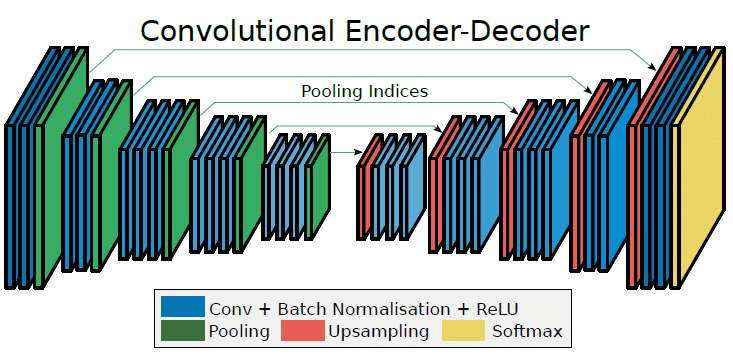
\includegraphics[width = 3.2in, height = 1.3in]{../images/segnet.png}}
    \caption{SegNet architecture}
    \label{segnet}
\end{figure}

\subsection{Cell counting}
After having segmented blood cell images masks for red, white blood cells and platelets, we use multiple post-processing methods to get the number of cells. All  algorithms we used to get a relatively accurate blood cell
count are as follow:
\subsubsection{Circle Hough Transform}
\hspace{\parindent}
Circle Hough Transform (CHT) is machine learning algorithm used to extract features (circles) from imperfect images.
We modified its parameters (Minimum distance, Minimum and Maximum radius...) for each type of blood cells (red, white and platelets).

We Modified this method by adding a loss function which will help us to eliminate False Positives circles by calculating the percentage of the intersection between the circle and the cell mask. We improve the counting accuracy by more than 20\% with a threshold intersection percentage of 60\%.

\subsubsection{Connected Component Labeling}
\hspace{\parindent}
Connected Component Labeling (CCL) is machine learning algorithm used to detect connected regions in a binary image.
Before applying the connected component labeling, we convert the images to gray-scale. Then, a binary threshold is applied to the images to get binary values.
Finally, we apply the connected component labeling to get the labels and map component labels to the resulting image, and the number of labels is the cell count accordingly.


\subsubsection{Watershed}
\hspace{\parindent}
In image processing, watershed algorithms—also known as drainage divide—are used largely for object segmentation, or separating up different objects in an image. The primary function of the watershed in this phase is to separate the touching and overlapping cells. To do this, the watershed requires two inputs. The first is an image with various intensity levels, in our case, the distance transform of our mask, where the intensity levels correspond to reliefs. In our situation, we retrieved local maxima from the distance transform picture for the second input, which is the water sources. we can see below the steps we used to count the cells.

\vspace*{-0.3cm}
\section{Experimentations and results}
\subsection{Dataset used in this work}
\subsubsection{Description}
The ALL-IDB1 dataset is a version of the ALL-IDB dataset, it is composed of 108 images (see figure \ref{img1}) collected in September 2005. The dataset consists of approximately 39,000 blood cells, with lymphocytes labeled by expert oncologists for identification and analysis \cite{labati2011all}. The images are all in JPG format, have a color depth of 24 bits, and are taken with a PowerShot G5 camera at a native resolution of 2592x1944. They depict various magnifications of a microscope, ranging from 300 to 500.

The ALL-IDB1 can be used for segmentation or classification with image processing methods or artificial intelligence models.

\begin{figure}
\centering
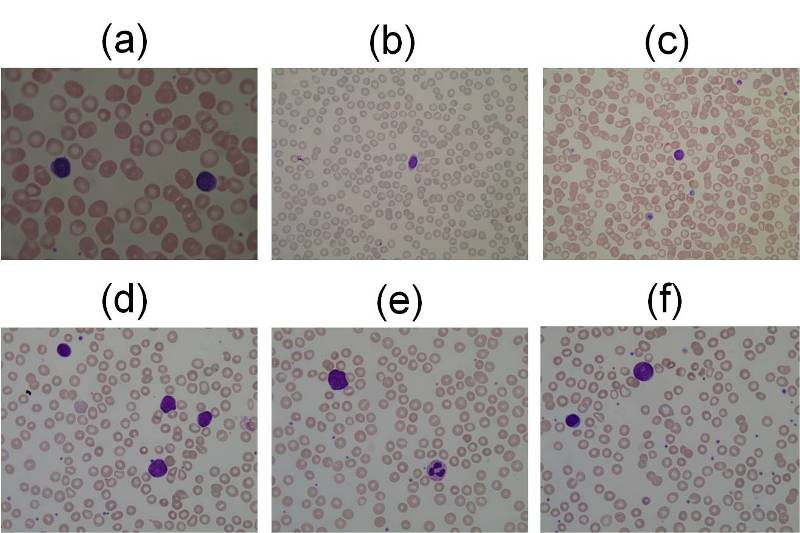
\includegraphics[width=3.5in,height=1.8in]{../images/ALLIDB1.jpg}
\caption{Examples of the images contained in ALL-IDB1: healthy cells from non-ALL patients (a,b,c), probable lymphoblasts from ALL patients (d,e,f). }
\label{img1}
\vspace*{-0.5cm}
\end{figure}

For both models, we decided to work with the updated ALL-IDB1 dataset which has 13 edge-masks and 108 masks of Red Blood Cells (RBCs), 108 masks of White Blood Cells (WBCs) and Platelets. For the count information we have 13 RBC images which have the count information, but for WBCs and Platelets we had to use manual count and algorithms to find the count information because they didn't provide the count information. For the WBC we used manual count, for the Platelets we used the connected component labeling on the ground truth mask.\\
10 images with their perspective masks and edge masks were chosen for red blood cell training and 3 as a test dataset, for white blood cells we used 73 images with their masks as a train dataset, and 33 as a test dataset.
For platelets, we used 71 images for training and 31 images as a test dataset.
The images will be sliced to the input size of the according model to match the input shape of the models, we also add a padding when we slice to recover the edges loss in convolution.

\subsubsection{Data augmentation}
We used the same dataset augmentation on all cells (red, white blood cells, and platelets) in both models UNet and SegNet.
The augmentation we used was custom which involves the following steps:
\begin{enumerate}
    \item Pick a random image from the train dataset.
    \item Get the x and y coordinates randomly from the chosen image.
    \item Rescale the image randomly to a smaller size then scale it back to the original size to reduce quality.
    \item Take a slice of the image and mask accordingly and also edge if available.
    \item Skip the image if it doesn't contain out object of interest
    \item Resize the image and mask to the model input.
    \item Randomly rotate and flip the image chip.
    \item Randomly augment the colors (luminosity and saturation).
\end{enumerate}
After data augmentation, we get 91060 images (tiles)  divided up as follows:
For red blood cells, the resulting train dataset will be 3916 image, mask, and edge tiles (a total of 11748 tiles) see table \ref{table:total_tiles}.For the test dataset 1072 image, mask, and edge tiles (a total of 3216 tiles).
For white blood cells, 28126 image and mask tiles were used for training (a total of 56252 tiles), and 15892 image and mask tiles were used as a test dataset for white blood cells (a total of 31784 tiles).
Finally, for platelets we used 27650 image and mask tiles were used for training (a total of 55300), and 14410 image and mask tiles as a test dataset for platelets (a total of 28820).\\
Table \ref{table:total_tiles}  contains the resulting sliced images for red blood cells, white blood cells and platelets .
\begin{table}[ht]
\centering
\resizebox{\columnwidth}{!}{%
\begin{tabular}{|cc|c|c|c|c|c|c|}
\hline
\multicolumn{2}{|c|}{{ \textbf{Dataset}}}                                                                     & { \textbf{\begin{tabular}[c]{@{}c@{}}Train\\ images\end{tabular}}} & { \textbf{\begin{tabular}[c]{@{}c@{}}Test\\ images\end{tabular}}} & { \textbf{\begin{tabular}[c]{@{}c@{}}Train\\ Tiles\end{tabular}}} & { \textbf{\begin{tabular}[c]{@{}c@{}}Test\\ Tiles\end{tabular}}} & { \textbf{\begin{tabular}[c]{@{}c@{}}Total\\ images\end{tabular}}} & { \textbf{\begin{tabular}[c]{@{}c@{}}Total\\ tiles\end{tabular}}} \\ \hline
\multicolumn{1}{|c|}{{ }}                                             & { \textbf{Image}} & { 10}                                                              & { 3}                                                              & { 3916}                                                           & { 1072}                                                          & { 13}                                                              & { \textbf{4988}}                                                  \\ \cline{2-8} 
\multicolumn{1}{|c|}{{ }}                                             & { \textbf{Mask}}  & { 10}                                                              & { 3}                                                              & { 3916}                                                           & { 1072}                                                          & { 13}                                                              & { \textbf{4988}}                                                  \\ \cline{2-8} 
\multicolumn{1}{|c|}{\multirow{-3}{*}{{ \textbf{Red Blood Cells}}}}   & { \textbf{Edge}}  & { 10}                                                              & { 3}                                                              & { 3916}                                                           & { 1072}                                                          & { 13}                                                              & { \textbf{4988}}                                                  \\ \hline
\multicolumn{1}{|c|}{{ }}                                             & { \textbf{Image}} & { 73}                                                              & { 33}                                                             & { 28126}                                                          & { 15892}                                                         & { 106}                                                             & { \textbf{44018}}                                                 \\ \cline{2-8} 
\multicolumn{1}{|c|}{\multirow{-2}{*}{{ \textbf{White Blood Cells}}}} & { \textbf{Mask}}  & { 73}                                                              & { 33}                                                             & { 28126}                                                          & { 15892}                                                         & { 106}                                                             & { \textbf{44018}}                                                 \\ \hline
\multicolumn{1}{|c|}{{ }}                                             & { \textbf{Image}} & { 71}                                                              & { 31}                                                             & { 27650}                                                          & { 14410}                                                         & { 102}                                                             & { \textbf{42060}}                                                 \\ \cline{2-8} 
\multicolumn{1}{|c|}{\multirow{-2}{*}{{ \textbf{Platelets}}}}         & { \textbf{Mask}}  & { 71}                                                              & { 31}                                                             & { 27650}                                                          & { 14410}                                                         & { 102}                                                             & { \textbf{42060}}                                                 \\ \hline
\end{tabular}%
}
\caption{Dataset used for both models}
\label{table:total_tiles}
\end{table}


\vspace*{-0.5cm}
\subsection{Metrics}
\begin{itemize}
    \item \textbf{Accuracy} Pixel accuracy It is the percent of pixels in the input image that are classified correctly as background or foreground.
    \item \textbf{IOU} The Jaccard Index or Intersection Over Union 
        \begin{equation}
        J(A,B) = \frac{Area\; of\; Overlap}{Area\; of\; Union} = \frac{|A \cap B|}{|A \cup B|}
        \end{equation}
    \item \textbf{Dice} aka. The Sørensen–Dice coefficient:
        \begin{equation}
            DSC = \frac{2 TP}{2 TP + FN + FP}
        \end{equation}
    \item \textbf{Tversky} The Tversky index :
        \begin{equation}
        S(X, Y) = 1-\frac{| X \cap Y |}{| X \cap Y | + \alpha|X \backslash Y| + \beta |Y \backslash X|}
        \end{equation}
\end{itemize}

\subsection{Results Discussion}
Most of the methods didn't focus on the counting side, the stop at the segmentation stage. In our method we did a full benchmark on the 3 blood components with 2 segmentation models and 3 counting algorithms.
For the segmentation we can see in the outputs that the SegNet gives better edge masks with sharp edges that helps removing the overlapping by subtraction. but i generates a lot of noise compared to U-Net which has no noise at all.

We have also a problem that affects both models which is the color space, if we change the colors a little bit in the input images we will get bad results because the models depends a lot on the RGB layers.

In the counting phase:
we had a problem the CHT algorithm where we was getting bad circles which doesn't cover any cell, we had to create a circle loss function to solve this problem with CHT.
in the watershed algorithm we get a lot of over-segmentation cases because of the shape and transparency of the WBCs.
for the 3 counting algorithms we had a parameter tuning problem, in our case we tuned the parameters manually. A summary of the results can be found in Table \ref{table:comparisonSegNet_UNet}


\subsection{DO-U-Net Results}
\subsubsection{Red Blood Cells}
\hspace{\parindent}
They are the most difficult to detect because of their nature of overlapping, where in some samples we can't see the overlapping by the naked eye, in this experiment we are testing the DO-U-Net from \cite{10.1007/978-3-030-44584-3_31}.
For the DO-U-Net we updated the data augmentation phase, and applied Transfer Learning to get a better edge-mask. we can see in the dataset that we only have 13 images out of 108 from ALL-IDB1 that contains edge-masks and 108 masks. Consequently, there is a lack of the edge-mask labels.
We ended up with the method below as the best fit to our problem:

\begin{enumerate}
    \item Train the DO-U-Net outputs on the large dataset (108 masks) which will output two identical masks.
    \item Continue Training the DO-U-Net with the small dataset (13 masks, 13 edges), and Freeze the Mask Output.
\end{enumerate}

\subsubsection{White Blood Cells}
\hspace{\parindent}
The White Blood Cells are also difficult to detect because of the non stable shape and in some cases they overlap, in this experiment we are comparing single output U-Net from \cite{10.1007/978-3-030-44584-3_31} and the single output SegNet model.
In the U-Net we removed the edge output because we don't have the edge annotation. then trained the model for 15 epochs with the binaryCrossEntropy Loss function on (74 + 34) images. 
We ended up with a very high accuracy and IOU score as we can see in table \ref{table:comparisonSegNet_UNet}.

\subsubsection{platelets}
\hspace{\parindent}
The platelets are easy to count because of the rare overlapping but they are a bit difficult to segment because of their small size.\\
In this experiment we are testing single output U-Net from \cite{10.1007/978-3-030-44584-3_31}. In the U-Net we removed the edge output because we don’t have the edge annotation.
then trained the model for 50 epochs with the BinaryCrossEntropy Loss function on (74 + 34) images.
We ended up with a very high accuracy and IOU score as we can see in table \ref{table:comparisonSegNet_UNet}.

\subsection{SegNet Results}
\hspace{\parindent}
SegNet segmentation results were pretty accurate for white blood cells and platelets, as for red blood cells, the segmentation was done using dual output (mask and edge-mask) to get rid of overlapped cells.\\
Here are the results of the Mean Squared Error (MSE) loss function on each type of cell:

\subsubsection{Red Blood Cells}
\hspace{\parindent}
For the dual-output SegNet model, the resulting segmented images were very good, sometimes better than the do-U-Net, though it is not as optimized when training and also predicting images, but it gets the job done with 95.86\% mask and 93.99\% edge accuracies. The segmented output images also had some noise which affected Connected Component Labeling (CCL) when counting.
As for Circle Hough Transform (CHT), the noise did not affect the result.
Red Blood Cells detection and counting is by far the hardest, because it is the only cell that overlaps and that makes it hard to count.
The segmented output of do-SegNet is thresholded using a binary threshold, and then sent to 3 algorithms:

\begin{itemize}
  \item \textbf{Circle Hough Transform}: CHT was our best result for red blood cells counting, which achieved an accuracy of 94.03\% on the same dataset used for training the model (13 images with their respective masks and edge-masks).
  \item \textbf{Connected Component Labeling}: CCL was applied directly on the thresholded output edge, this method was far from accurate because the do-SegNet output had some noise (even when removing most of it), and also the overlapped nature of red blood cells which makes it very hard for this algorithm to count correctly. CCL achieved an accuracy of 76.49\% counting red blood cells.
  \item \textbf{Euclidean Distance Transform}: EDT is used to get rid of the overlapped cells, also peak local max was applied on the EDT output for finding local maxima(s), the result of this approach is 84.64\% accuracy.
\end{itemize}

\subsubsection{White Blood Cells}
\hspace{\parindent}
The results of white blood cells segmentation and counting using the SegNet model was very accurate achieving 99.72\% when segmenting.
White blood cells are the easiest out of the three, and the most accurate results.
However, white blood cells are different from the other cells because they come in different shapes and sizes, which made it hard to adapt each counting algorithm to every cell.\\
The same counting methods are applied CHT, CCL and EDT. And each method had some drawbacks.\\
Here are the results:
\begin{itemize}
  \item \textbf{Circle Hough Transform}: Due to the different shapes of white blood cells, CHT achieved the lowest result which is 79.9\% counting accuracy, because some of the cells don't even look like circles and also their different size which made it harder to count.
  \item \textbf{Connected Component Labeling}: CCL is similar to CHT when it comes to white blood cells. And, because of the noisy outputs of SegNet the binary threshold can only do so much (it thresholds some of the noise generated when predicting).\\
    CCl achieved an average counting accuracy of 82.89\%.
  \item \textbf{Euclidean Distance Transform}: EDT is the contender of white blood cells counting, because the distance transform gets rid of the noise completely and peak local max was very helpful in eliminating that noise and getting an accurate count.\\
    This method achieved a counting accuracy of 96.43\%.
\end{itemize}

\subsubsection{Platelets}
\hspace{\parindent}
The platelets segmentation result we achieved is not the best compared to the do-U-Net model. SegNet extracts the platelets but with some noise which made it very hard to count accurately.
It achieved a segmentation accuracy of 99.89\% and the highest counting accuracy is 71.56\% which is not very good.\\
Here are all the counting accuracies for each approach:

\begin{table*}[t]
\centering
\resizebox{\textwidth}{!}{%
\begin{tabular}{|c|c|cccc|cccc|}
\hline
\multirow{3}{*}{\textbf{\begin{tabular}[c]{@{}c@{}}Blood Cells\\ / Model\end{tabular}}} & \multirow{3}{*}{\textbf{Output}} & \multicolumn{4}{c|}{\textbf{DO-U-Net}}                                                                                                                                                               & \multicolumn{4}{c|}{\textbf{SegNet}}                                                                                                                                                        \\ \cline{3-10} 
                                                                                        &                                  & \multicolumn{1}{c|}{\multirow{2}{*}{\textbf{Segmetation Accuracy \%}}} & \multicolumn{3}{c|}{\textbf{Counting Accuracy \%}}                                                                          & \multicolumn{1}{c|}{\multirow{2}{*}{\textbf{Segmetation Accuracy \%}}} & \multicolumn{3}{c|}{\textbf{Counting Accuracy \%}}                                                                 \\ \cline{4-6} \cline{8-10} 
                                                                                        &                                  & \multicolumn{1}{c|}{}                                                  & \multicolumn{1}{c|}{\textbf{CHT}}                    & \multicolumn{1}{c|}{\textbf{CCL}}           & \textbf{Watershed}     & \multicolumn{1}{c|}{}                                                  & \multicolumn{1}{c|}{\textbf{CHT}}           & \multicolumn{1}{c|}{\textbf{CCL}}           & \textbf{Watershed}     \\ \hline
\multirow{2}{*}{\textbf{\begin{tabular}[c]{@{}c@{}}Red Blood\\ Cells\end{tabular}}}     & \textbf{Mask}                    & \multicolumn{1}{c|}{\textbf{97.16}}                                    & \multicolumn{1}{c|}{\multirow{2}{*}{\textbf{95.36}}} & \multicolumn{1}{c|}{\multirow{2}{*}{78.66}} & \multirow{2}{*}{90.43} & \multicolumn{1}{c|}{95.86}                                             & \multicolumn{1}{c|}{\multirow{2}{*}{94.03}} & \multicolumn{1}{c|}{\multirow{2}{*}{76.49}} & \multirow{2}{*}{84.64} \\ \cline{2-3} \cline{7-7}
                                                                                        & \textbf{Edge}                    & \multicolumn{1}{c|}{93.85}                                             & \multicolumn{1}{c|}{}                                & \multicolumn{1}{c|}{}                       &                        & \multicolumn{1}{c|}{\textbf{93.99}}                                    & \multicolumn{1}{c|}{}                       & \multicolumn{1}{c|}{}                       &                        \\ \hline
\textbf{\begin{tabular}[c]{@{}c@{}}White Blood\\ Cells\end{tabular}}                    & \textbf{Mask}                    & \multicolumn{1}{c|}{\textbf{99.76}}                                    & \multicolumn{1}{c|}{88.7}                            & \multicolumn{1}{c|}{58.74}                  & \textbf{97.94}         & \multicolumn{1}{c|}{99.72}                                             & \multicolumn{1}{c|}{79.9}                   & \multicolumn{1}{c|}{82.89}                  & 96.43                  \\ \hline
\textbf{Platelets}                                                                      & \textbf{Mask}                    & \multicolumn{1}{c|}{99.46}                                             & \multicolumn{1}{c|}{X}                               & \multicolumn{1}{c|}{\textbf{98.58}}         & X                      & \multicolumn{1}{c|}{\textbf{99.89}}                                    & \multicolumn{1}{c|}{65.65}                  & \multicolumn{1}{c|}{71.56}                  & 65.65                  \\ \hline
\end{tabular}%
}
\caption{Comparison of DO-U-Net and SegNet results}
\label{table:comparisonSegNet_UNet}
\end{table*}


\subsection{Result samples}
\hspace{\parindent}
Here is the resulting output of each model on Im037.jpg (see figure \ref{fig:originalImage}), segmenting all the cells Red, White and platelets:
\vspace*{-0.5cm}
\begin{figure}[ht]
  \centering
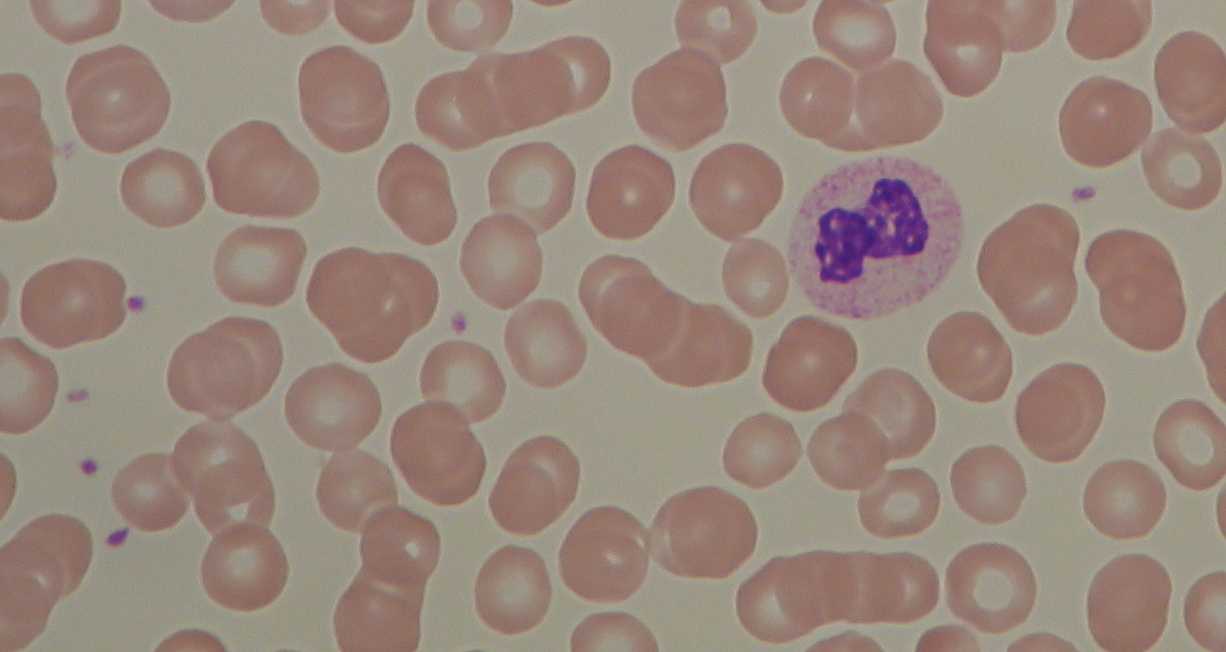
\includegraphics[width = 5cm,height=2.5cm]{../images/originalCHT.jpg}
  \caption{Original image Im037.jpg}
  \label{fig:originalImage}
    \vspace*{-0.7cm}
\end{figure}

\begin{figure}[ht]
  \centering
  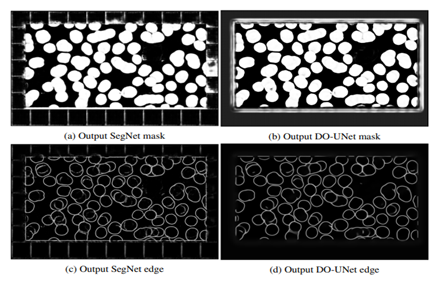
\includegraphics[width = 3.5in,height=2in]{../images/rbc.png}
  \caption{Output from SegNet and DO-UNet segmenting Red Blood Cells}
  \label{fig:rbc}
  \vspace*{-0.5cm}
\end{figure}

\begin{figure}[ht]
  \centering
  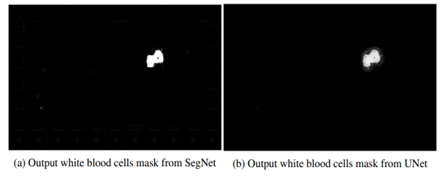
\includegraphics[width = 3.5in,height=1in]{../images/wbc.png}
  \caption{Outputs from SegNet and UNet segmenting White Blood Cells}
  \label{fig:wbc}
    \vspace*{-0.3cm}
\end{figure}

\begin{figure}[ht]
  \centering
  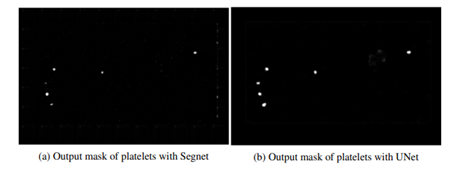
\includegraphics[width = 3.5in,height=1in]{../images/plt.png}
  \caption{Outputs from SegNet and UNet segmenting platelets}
  \label{fig:plts}
    \vspace*{-0.5cm}
\end{figure}

After all the steps we have mentioned above, the final output of each counting algorithm is presented in the figures below:

\begin{itemize}
  \item \textbf{Figure \ref{fig:ccl_output}} (a): Circle Hough Transform applied on the segmented output of Red Blood Cells, the CHT method performed very well on the edge output of the do-U-Net model.
    Because of the circular shape of red blood cells and the parameter tuning of CHT, this is the best counting accuracy we achieved on Red Blood Cells.
  \item \textbf{Figure \ref{fig:ccl_output}} (b): Watershed applied on the segmented output of White Blood Cells. Watershed outperformed the other algorithms because it segments touched and overlapped objects. this is the best counting accuracy we achieved on White Blood Cells.
  \item \textbf{Figure \ref{fig:ccl_output}} (c): Connected Component Labeling applied on the segmented output of White Blood Cells. This method performed well when it came to none touching objects (Platelets), in this figure also 2 Platelets where also detected as White Blood Cells, but they will get removed using the surface filter we implemented, which gets rid of small objects.
\end{itemize}

\vspace*{-0.4cm}
\begin{figure}[ht]
  \centering
  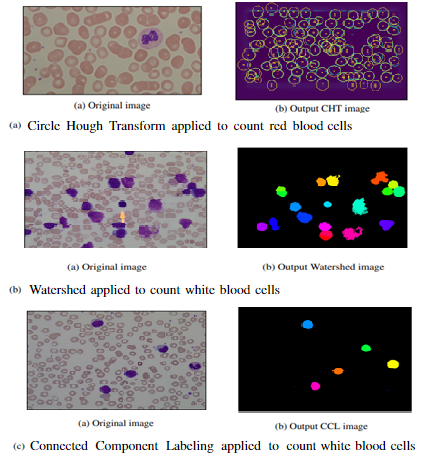
\includegraphics[width = 3.5in,height=3.3in]{../images/result.png}
  \caption{Connected Component Labeling applied to count white blood cells}
  \label{fig:ccl_output}
    \vspace*{-0.5cm}
\end{figure}
  \vspace*{-0.2cm}
\section{Conclusion}

In the present work, we have mainly presented two different models of segmentation based on CNNs and three counting algorithms to perform a complete blood count.
We focused more on the segmentation task where  we tested two models U-Net and SegNet to get better masks. 

We can see that the U-Net gave better result with less noisy mask, but the two models has some weaknesses with the images color space, because both models takes RGB images therefore they depend a lot on the color features.

In the counting task, we had a small time window where we could not tune the 3 three algorithm parameters to get the best results. but we got acceptable results in each blood cell type, especially with platelets.

As a future work, we can combine between the two models to benefit the strength points of both models, we can also find more combinations between edge and mask.
We can Also create a model that predicts the algorithm parameters for watershed and CCL rather than tuned it manually. 

\bibliographystyle{IEEEtran}
\bibliography{main}

\end{document}
